\section{Overview of \vtkm}
\label{sec:overview}

%\assign{Hank, editting pass (perhaps trimming)}

The \vtkm library~\citep{Moreland2016} began as a research project funded
by the 
Advanced Scientific Computing Research program within the US Department of Energy's (DOE's) Office of Science.
The project's goal was to enable scientific visualization on emerging high-performance computing (HPC) systems via
two approaches:
(1)~by serving as a repository for interoperable scientific visualization algorithms well suited to accelerator architectures and (2)~by providing a framework that simplifies the development of visualization algorithms that can be ported across many accelerator devices.

%\ken{Idea from Jay: summarize the filters and stuff we have done in a table so that people can easily add their work.}

%\jay{Table is added and we might simplify this paragraph a little bit and put detailed references into the table.}

At the onset of the ECP, \vtkm contained only the most common operations for scientific visualization: contour, threshold, external faces, basic surface simplification, and rendering.
Although this initial set of operations is useful, users almost always require more functionality.
The ECP enabled this additional functionality to grow with the introduction of new algorithms and performance improvements to the existing ones.
Table~\ref{tab:algorithms} contains a selection of algorithms currently provided by \vtkm.
These added features provided the necessary functionality for the tools and applications that utilized \vtkm to execute on exascale machines and similar hardware.

%% \begin{figure}[htb]
%%   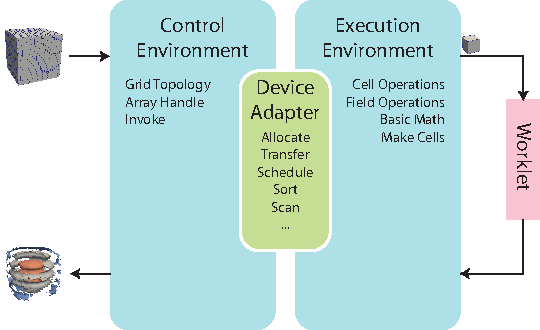
\includegraphics[width=\linewidth]{vtkm-framework}
%%   \caption{The basic \vtkm framework for device portability. \hank{Do we have a copyright issue with using this image?  Has it appeared before?} \ken{I'm not totally sure. For now, let's delete it and use something else instead.}}
%%   \label{fig:vtkm-framework}
%% \end{figure}

%The basic structure for \vtkm's framework is shown in Figure~\ref{fig:vtkm-framework}.
The basic workflow for an algorithm in \vtkm's framework is shown in Figure~\ref{fig:vtkm-workflow}.
%\vtkm provides a framework designed for optimizing both developer time and execution time on
%diverse many-core devices.
The framework separates code into two environments: control and execution.
In a GPU development environment, control corresponds to the ``host,'' and execution corresponds to the ``device.''
This separation is maintained even when 
there is not a clear separation between host and device, which is the case for some accelerators such as the Xeon Phi~\citep{Jeffers2016}.

Algorithms in \vtkm execute parallel routines by wrapping them in a functional object that will be passed to the device in the execution environment. There, it will be run on many threads, and each instance will be fed a small, isolated portion of the data.
This functional object is called a ``worklet'' because it works on a small portion of data.
The worklet API in the execution environment is designed to promote thread safety to simplify the implementation and to prevent memory access hazards.
%This design promotes developer efficiency, as
%\vtkm simplifies implementations for current and future algorithms, and also provides 
%automatic and efficient porting of these algorithms across different devices.
It is also well suited for modern devices that require many (thousands or more) parallel threads to run efficiently, which are the type of devices \vtkm is designed for.

To achieve portability, \vtkm contains a device adapter that manages interaction with a variety of devices.
The entirety of \vtkm can be ported with a change to the device adapter.
%
Furthermore, all execution code (``device code'') is implemented with standard C++14
%and thus universal for any GPU device.
and can thus be compiled for any device supporting this very common programming environment.
%\hank{Is this statement too strong?}
%\ken{I've qualified the statement to be more accurate. I am leaving out some qualifications about using only the subset of the language supported by the device compiler, but would that much detail be necessary here?}

\vtkm uses multiple techniques to achieve efficient parallelization.
One technique is
to enable data to be divided into small pieces for parallel execution by
using a 
flexible data model~\citep{Meredith2012}.
A second technique is
to utilize
data parallel primitive methods~\citep{Blelloch1990}.
Data parallel primitives allow algorithms to be implemented as a sequence of data parallel operations such as map, scan, sort, and reduce.
Early work explored how to implement scientific visualization using data parellel primitives~\citep{Lo2012}.
Map applies an operation to each datum and is a convenient way to specify parallel operations.
Scan, which produces a running sum, product, or other associative operation, is useful for building indicies after counting.
Sort reorders data to make duplicates easy to find.
Reduce provides a total sum or product for quick accumulations.

To simplify the implementation further, \vtkm provides meta data-parallel primitives~\citep{Moreland2021} that incorporate common patterns for scientific data that were demonstrated to be efficient.
For example, \vtkm provides a meta data-parallel primitive to map an operation to every cell of a mesh while internally handling all the indexing of shape and incident point information.
Finally, note that the \vtkm design achieves developer efficiency with 
streamlined algorithm development and 
automatic
porting to new architectures with an efficient implementation.
